\section{Introduction}
\label{sec:intro}

Charged lepton flavor violating (CLFV) processes, such as 
$\mu^+\to e^+\gamma$ and $\mu^+\to e^+e^-e^+$, are mediated by neutrino oscillations in loop diagrams in the Standard Model (SM). While allowed, these reactions are highly suppressed due to the extremely small neutrino masses. For example, the branching fraction for $\mu \to e \gamma$ is given by~\cite{xxx}
\begin{equation}
BR(\mu \rightarrow e \gamma)=\frac{3\alpha}{32\pi}\left|\sum_i U_{\mu
i}^* U_{e i}\frac{m_{\nu_{i}}^2}{m_{W}^2}\right|^2 \sim 10^{-52},
\end{equation}
where $U_{ei}$ are the leptonic mixing matrix elements, assuming neutrinos
are Dirac particles. This is clearly well below the reach of any conceivable experiment.
However, in many extensions of the SM, such as supersymmetric grand unified
theories or theories with extra dimentions, larger contributions to CLFV are
allowed~\cite{new physics}. Observing CLFV is therefore a clear indication of physics beyond the Standard Model (henceforth BSM physics). Figure~\ref{CL:mutoegamma} shows an example of BSM processes mediated by SUSY particles.

The effective Lagrangian relevant for the $\mu^+\to e^+\gamma$ and $\mu^+\to e^+e^-e^+$
decays can be parametrized, regardless of the origin of CLFV, as a sum of
dipole terms and a ``contact term''. The $\mu^+\to e^+\gamma$ process is only sensitive to the dipole terms, while both dipole and contact terms contribute to $\mu^+\to e^+e^-e^+$ decays~\cite{deGouvea:2013zba}. Improving upper limits of
the $\mu^+\to e^+\gamma$ and $\mu^+\to e^+e^-e^+$ branching fractions down to $10^{-14}$ and $10^{-16}$, respectively, could probe scales of BSM physics up to several thousands of TeV. In addition, the Dalitz plot of the $\mu \rightarrow eee$ decays offers the possibility to determine the chirality of BSM physics, should it be observed with sufficient statistics~\cite{Okada:1999zk}. 

\begin{figure}[htbp]
\begin{center}
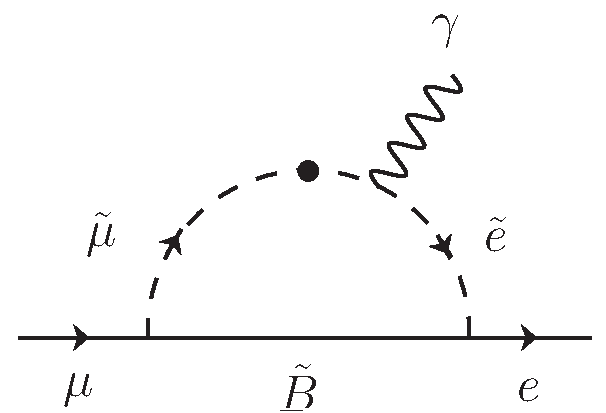
\includegraphics[width=5cm]{Figures/mu_e_gamma_diagram.pdf} \hspace*{2cm}
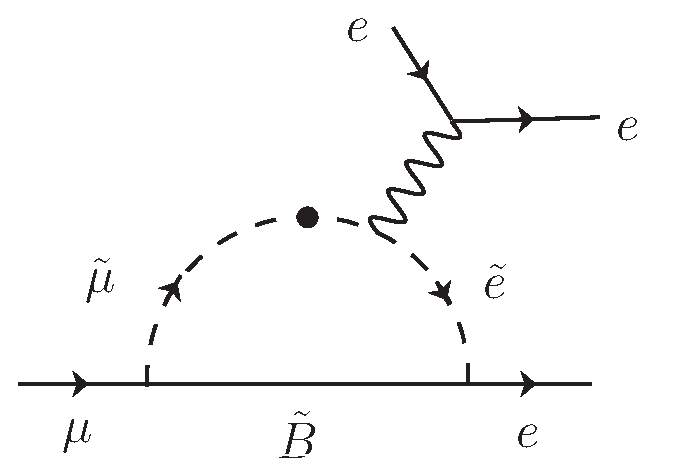
\includegraphics[width=5cm]{Figures/mu_3e_diagram.pdf}
\caption{\label{CL:mutoegamma}$\mu \rightarrow e\gamma$ decay mediated by SUSY particles (left panel), and $\mu \rightarrow 3e$ decay (right panel).}
\end{center}
\end{figure}

We discuss herein feasibility studies of next generation detectors designed to search for $\mu^+\to e^+\gamma$ and $\mu^+\to e^+e^-e^+$ decay that could be performed at Fermilab during Project X era. These searches complement improved searches for $\mu \to e$ conversion that could also be done at Project X~\cite{Mu2eII}.



